%%%%%%%%%%%%%%%%%%%% author.tex %%%%%%%%%%%%%%%%%%%%%%%%%%%%%%%%%%%
%
% sample root file for your "contribution" to a proceedings volume
%
% Use this file as a template for your own input.
%
%%%%%%%%%%%%%%%% Springer %%%%%%%%%%%%%%%%%%%%%%%%%%%%%%%%%%


\documentclass{svproc}
%
% RECOMMENDED %%%%%%%%%%%%%%%%%%%%%%%%%%%%%%%%%%%%%%%%%%%%%%%%%%%
%

% to typeset URLs, URIs, and DOIs
\usepackage{url}
\usepackage[english]{babel}
\selectlanguage{english}
\usepackage[utf8]{inputenc}
\usepackage{graphicx}    % can use native umlauts

\def\UrlFont{\rmfamily}

\begin{document}
\mainmatter              % start of a contribution
%
\title{Applying Machine Learning to Investigate Effects of contaminated PCR Plates in a Metagenomic Sequencing Study}
%
\titlerunning{Effects of contaminated PCR plates}  % abbreviated title (for running head)
%                                     also used for the TOC unless
%                                     \toctitle is used
%
\author{Maximilian Joas\inst{1} }
%
%\authorrunning{$<$Joas$>$ et al.} % abbreviated author list (for running head)
%
%%%% list of authors for the TOC (use if author list has to be modified)
\tocauthor{Maximilian Joas}
%
\institute{Universität Leipzig\\Machine Learning Group\\Leipzig, Germany\\
\email{mj13body@studserv.uni-leipzig.de}}
%
\maketitle              % typeset the title of the contribution
%
\begin{abstract}
  The objectives of this work are to predict contaminated PCR plates based on OTU read counts and to investigate specific characteristics of the contaminated plates. A random forest classifier and MLP were used to predict the plate as well as to find important characteristics of the contaminated plate. The prediction resulted in an accuracy of 0.84 and important OTUs had higher read counts than non-important ones. In conclusion, it is possible to predict contaminated PCR plates with machine learning based on OTU counts.
   \keywords{Machine Learning, Empirical Data, Scientific Research}
\end{abstract}
%
%
\section{Research Question}
%
Metagenomics an area of research that studies genetic material obtained directly from environmental samples.
Advances and cost reduction of sequencing experiments had a great impact on the field of Metagenomics.
The vast amount of data obtained from whole-genome sequencing experiments in metagenomic leads to opportunities in pathogen detection, ecological studies and drug development \cite{THREE OPNE TABS}. On the other hand, the abundance of data poses challenges to the analysis of metagenomic data. Consequently, classical statistical methods reach their limits and other approaches such as machine learning are often used \cite{Soueidan2017}.\\


Not only the amount of data but also the type of data are challenging, on top of that, the technical process of sequencing can lead to problems.
In particular, contamination and noise are important problems when studying metagenomics \cite{paper Michel}. Noised up and or contaminated data can lead to false conclusions in experiments. Therefore it would be valuable to predict contamination on PCR plates and find factors that are distinctive to contaminated PCR plates. In this work, I will investigate if it is possible to predict contaminated PCR plates based on OTU counts as well as metadata. Furthermore, I will present factors that distinguish contaminated from not contaminated PCR plates with the help of machine learning.


\section{State of the Art}
Machine learning methods have been successfully used in the study of metagenomics data  \cite{Soueidan2017}. However, specifically on this research question, there are, to the best of my knowledge no publications. Nevertheless, this section aims to give an overview of the state of the art of the implemented methods. TODO paper zusammenfassen

%
%
\section{Methods}
%
\subsection{Conception}

The research question is divided into two parts: (I) Is it possible to predict the contaminated PCR plate? (II) What did change on the contaminated PCR plates? \\
The first question is a typical problem for a supervised learning approach: I used two methods to predict the PCR Plate, one classical machine learning approach (Random Forest Classifier) and a neuro-inspired approach (Multi-Layer Perceptron).  Additionally, a dummy classifier and a decision tree classifier was used to set the prediction of the complex methods into context.
In order to solve the second question in a machine learning context, the most important features for the supervised learning method were retrieved. Therefore, I had to use methods that not only predict the contaminated plate but also determine the most important features for the prediction. The random forest Gini importance was used as a measurement together with the Shapely value
Both research questions have been examined with a dataset comprising of OTU count data and the corresponding metadata, which is presented in the following section.

\subsection{Data and Preprocessing}

The data set was provided by the ETH Zurich. The data consisted of a count table of microorganisms sequencing reads from mice from different laboratories The data set did not come normalized. Additionally, to the count table, a data set containing metadata was included in the analysis. The metadata contained a variety of technical information, such as the PCR plate, the date of the extraction run, or the name of the researchers that executed the experiments. In total, the data set consisted of 199 samples and 1564 OTUs and 61 different metadata entries per sample. The median sequencing depth of the samples was 80275. Note that the ETH Zurich provided another dataset with three replicas of each sample, but for the analyses, the dataset without the replicas was used.\\
Firstly, 17 non-informative features, that had additionally an abundance of missing values, were excluded manually from the metadata. Subsequently, I aggregated the information about the PCR plate by grouping the not-contaminated plates together. This resulted in a binary classification problem. The count-table did not contain any missing values, the metadata had multiple features with missing values. When the metadata was used for the prediction, I excluded samples with missing values. 26 samples were excluded from this experiment. Subsequently, the datatype was checked, non-numeric data types were transformed to ordinal values. In contrast to one-hot encoding this method does not increase the feature space. However, it can have an influence on the predictions. 
Lastly, I checked for outlines in the metadata via Boxplots but did not find too extreme values that had to be excluded. For the count-table a z-transformation was performed, in order to use it for the multilayer perceptron. A closer description of the implementation follows in the next subsection.

\subsection{Supervised Learning Methods}
In order to predict the contaminated class, the relative frequency of the more frequent class was established as a dummy classifier for comparison. Subsequently, a decision tree was used as baseline classifier. The default parameters where used from the decision tree implementation of the python package scikit-learn\footnote{https://scikit-learn.org/stable/index.html} v.0.23.2. Specifically the following parameters were used: TODO

In order to evaluate the decision tree, I used ten-fold cross-validation and the Accuracy, Precision, Recall and F1 Score as the evaluation metric.
Subsequently, a more with the random forest classifier a more complex model was used to predict the contamination. Therefore the random forest classifier of scikit-learn was implemented with the default parameters as seen in table XX. The evaluation followed
Since the latter two methods are statistically inspired, a neuro-inspired approach was implemented in addition. Hereford a multilayer perceptron was implemented with the default parameters of the python package sckit-learn v.0.23.2 as seen in table XX.\\

In order to answer the second research question - what was different on the contaminated plate - the goal was to find features that are associated with the prediction of the contaminated plate. Therefore, the Gini importance of the random classifier was used. Additionally, the Shapley values of the features were calculated based on the trained random forest. The shaply value is a metric for the contribution of a feature to the prediction. TODO SHAPLEY BETTER AS GINI For the feature importance, the data was split with a 70/30 ratio into training and test data. Class balances were controlled for the two datasets. All analyses, except for the MLP were performed for the count data and the metadata. The results are presented in the following section.
\section{Results}
The results of the two research questions are presented separately Firstly the results of the prediction of the PCR plate are presented.
\subsection{Prediction of the PCR plate}
The dummy classifier, defined as the relative frequency of the more frequent class, was 0.52. Firstly, the results prediction with the count data is presented: A decision tree served as a baseline classifier yielded an accuracy of 0.67. Additional evaluation metrics like Precision, Recall and F1 score can be found in table XX. The training with a test and validation set of the random forest resulted in an accuracy of 0.87. The average evaluation metrics for the tenfold cross-validation of the random forest and the MLP can also be found in table XX. The MLP did beat the dummy classifier but had with 0.67 no higher accuracy than the baseline decision tree classifier. \\
When using the metadata as features to predict the contaminated plate all evaluation metrics resulted in a perfect prediction (Accuracy:1, Precision:1, Recall:1, F1 score: 1).
\begin{table}
   \caption{Evaluation metrics for the prediction of the PCR plate}
   \begin{center}
       \begin{tabular}{l@{\quad}lllll}
           \hline
         
                  Method & Accuracy & Precision & Recall & F1 Score\\[2pt]
                                   \hline\rule{0pt}{12pt}
                   Decision Tree  &    0.67 & 0.62 & 0.71 & 0.67 \\
                   Random Forest &    0.84 & 0.93 & 0.74 & 0.75 \\
                   MLP   &    0.66 & 0.63 & 0.68 & 0.59 \\
                   [2pt]
                   \hline
       \end{tabular}
   \end{center}x
   \label{tab1}
\end{table}


\subsection{Features of the contaminated PCR plate}
In order to investigate differences between contaminated and non-contaminated plates, the ten most important features according to the random forest Gini importance were extracted for the count data and the metadata. The exact taxonomy of the corresponding OTUs can be found in the data (published on GitLab along with scripts) Since there were no notable differences between the Shapley value and the Gini importance, only results of the Gini importance are reported.
The most important metadata features were the date of the 16S PCR, the extraction run and the library prep attempt. The ten most important OTUs are shown in Figure 1C. Figures 1A and 1B show a beeswarmplot of counts of the ten most and ten least important features. A notable difference is the number of counts. The most important OTUs had on average higher count numbers.

\begin{figure}
		
		
		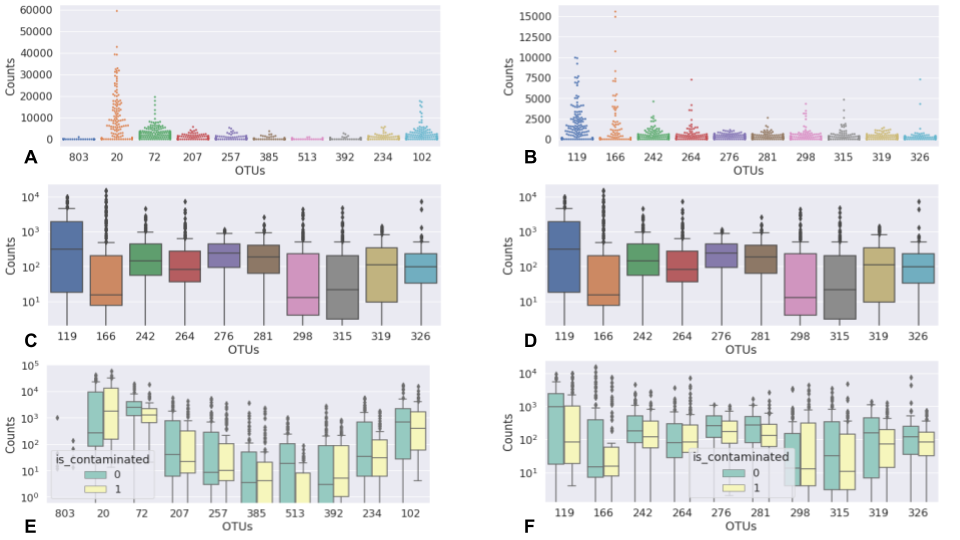
\includegraphics[ scale = 0.4]{./figs/plotsPraktikum.png}
		\caption{A: Beeswarmplot of counts of the ten most important OTUs according to Gini importance. B analogous to A for the ten least important features. C Barplot of the Gini importance of the ten most important OTUs}
	\end{figure}


\section{Discussion}
The results of the prediction of the PCR plates seem plausible for the analyses with the count data. The results as shown in table XX reveal that a more complex MLP is not superior to the simple decision tree. However, when using statistically inspired models the complex random forest is superior to the decision tree in all metrics. The comparatively small value of the recall of the random forest classifier implies a higher number of false negatives. Since the presented analyses were highly specific to the data and question there are not existing reference metrics from other publications. However, in a general machine learning context, the results are reasonable. It should be noted that none of the parameters of the methods were tuned. The comparatively low accuracy of the MLP could be also contributed to this lack of tuning. The lack of parameter tuning could be seen as a major limitation of this work. However, the predictions of the tree-based models resulted in accurate predictions and could therefore be used to extract important features even without tuning.
The fact that the prediction with the metadata yielded perfect predictions seems highly unplausible at first sight. On the other hand, the information about the PCR plate of the sample could be encoded in other metadata features. e.g plate one was performed on certain days. This could also be observed when contemplating the feature importance where the date of the 16s PCR step was the most important feature.
The analyses of the OTU importance showed that important OTUs had higher count numbers than unimportant ones. One could argue that this is due to the higher absolute values, but random forest classifiers are known to deal well with unscaled data. Another aspect that have to be considered is that the contamination needs to be somehow visible. Consequently it is only logical that the contaminated plates had on average higher count numbers.
 In general, it is hard to draw a causal conclusion about specific contaminations, because I assumed the samples were distributed randomly across the PCR plates, which is not generally the case.
  
%
%
\section{Conclusion}
%
In summary, it is possible to predict the contaminated plate with the OTU count data. A random forest classifier yields the most accurate predictions but has a comparatively high false-negative rate. Additionall, OTUs were found that predicted the contaminated plate particularly well.Hence there could be found a difference between contaminated and non-contaminated PCR plates: Prediction relevant OTUs had on average higher count numbers than the ones that did not have an influence on the prediction of the contamination. It remains subject to future research, if contaminated plates hava always higher count numbers than non-contamined plates. In this work machine learning and a neuro-inspired approach were used. A comparison with a Bayesian approach could be interesting in further studies.

%
% ---- Bibliography ----
%
%
\bibliographystyle{plain}
\bibliography{Paperrunde.bib}


\end{document}


